\documentclass{chi-ext}
% Please be sure that you have the dependencies (i.e., additional LaTeX packages) to compile this example.
% See http://personales.upv.es/luileito/chiext/

%% EXAMPLE BEGIN -- HOW TO OVERRIDE THE DEFAULT COPYRIGHT STRIP -- (July 22, 2013 - Paul Baumann)
% \copyrightinfo{Permission to make digital or hard copies of all or part of this work for personal or classroom use is granted without fee provided that copies are not made or distributed for profit or commercial advantage and that copies bear this notice and the full citation on the first page. Copyrights for components of this work owned by others than ACM must be honored. Abstracting with credit is permitted. To copy otherwise, or republish, to post on servers or to redistribute to lists, requires prior specific permission and/or a fee. Request permissions from permissions@acm.org. \\
% {\emph{CHI'14}}, April 26--May 1, 2014, Toronto, Canada. \\
% Copyright \copyright~2014 ACM ISBN/14/04...\$15.00. \\
% DOI string from ACM form confirmation}
%% EXAMPLE END -- HOW TO OVERRIDE THE DEFAULT COPYRIGHT STRIP -- (July 22, 2013 - Paul Baumann)

\title{CCRec: Content of Publications and Collaboration Network Combined Academic Collaboration Recommendation}



\numberofauthors{6}
% Notice how author names are alternately typesetted to appear ordered in 2-column format;
% i.e., the first 4 autors on the first column and the other 4 auhors on the second column.
% Actually, it's up to you to strictly adhere to this author notation.
\author{
  \alignauthor{
  	\textbf{First Author}\\
  	\affaddr{AuthorCo, Inc.}\\
  	\affaddr{123 Author Ave.}\\
  	\affaddr{Authortown, PA 54321 USA}\\
  	\email{author1@anotherco.com}
  }\alignauthor{
  	\textbf{Fourth Author}\\
  	\affaddr{AuthorCo, Inc.}\\
  	\affaddr{123 Author Ave.}\\
  	\affaddr{Authortown, PA 54321 USA}\\
  	\email{author5@anotherco.com}
  }
  \vfil
  \alignauthor{
  	\textbf{Second Author}\\
  	\affaddr{AuthorCo, Inc.}\\
  	\affaddr{123 Author Ave.}\\
  	\affaddr{Authortown, PA 54321 USA}\\
  	\email{author2@anotherco.com}
  }\alignauthor{
  	\textbf{Fifth Author}\\
  	\affaddr{AuthorCo, Inc.}\\
  	\affaddr{123 Author Ave.}\\
  	\affaddr{Authortown, PA 54321 USA}\\
  	\email{author6@anotherco.com}
  }
  \vfil
  \alignauthor{
  	\textbf{Third Author}\\
  	\affaddr{AuthorCo, Inc.}\\
  	\affaddr{123 Author Ave.}\\
  	\affaddr{Authortown, PA 54321 USA}\\
  	\email{author3@anotherco.com}
  }\alignauthor{
  	\textbf{Sixth Author}\\
  	\affaddr{AuthorCo, Inc.}\\
  	\affaddr{123 Author Ave.}\\
  	\affaddr{Authortown, PA 54321 USA}\\
  	\email{author7@anotherco.com}
  }
}

% Paper metadata (use plain text, for PDF inclusion and later re-using, if desired)
\def\plaintitle{CHI LaTeX Extended Abstracts Template}
\def\plainauthor{Luis A. Leiva}
\def\plainkeywords{Guides, instructions, author's kit, conference publications}
\def\plaingeneralterms{Documentation, Standardization}

\hypersetup{
  % Your metadata go here
  pdftitle={\plaintitle},
  pdfauthor={\plainauthor},
  pdfkeywords={\plainkeywords},
  pdfsubject={\plaingeneralterms},
  % Quick access to color overriding:
  %citecolor=black,
  %linkcolor=black,
  %menucolor=black,
  %urlcolor=black,
}

\usepackage{graphicx}   % for EPS use the graphics package instead
\usepackage{balance}    % useful for balancing the last columns
\usepackage{bibspacing} % save vertical space in references
\usepackage{subfigure}
\usepackage{epstopdf}


\begin{document}

\maketitle

\begin{abstract}
With the academic research filed expanding, the problem of finding proper potential collaborators is really cumbersome. In this paper, we proposed a content of publications and collaboration network combined academic Collaboration recommendation model (CCRec). Compared to traditional approaches, CCRec is more effective because it recommends collaborators combining the content of publications and collaboration network in different topics. Experiments based on DBLP data sets show that CCRec significantly outperforms traditional approaches, with the topic drift problem well solved.
\end{abstract}

\keywords{\plainkeywords}
\textcolor{red}{Mandatory section to be included in your final version.}

\category{H.5.m}{Information interfaces and presentation (e.g., HCI)}{Miscellaneous}.
%See \cite{ACMCCS}
See: \url{http://www.acm.org/about/class/1998/}
for help using the ACM Classification system.
\textcolor{red}{Mandatory section to be included in your final version.}

%\terms{\plaingeneralterms}
%\textcolor{red}{Optional section to be included in your final version.}


% =============================================================================
\section{Introduction}
% =============================================================================
Collaboration network is one kind of academic social networks formed by researchers and their collaborations. In the academic field, recommending collaborators to researchers (groups) may help researchers build more collaborations and become more prolific.

Some Studies proposed to recommend academic collaborators by exploiting the collaboration network and the profiles of researchers such as affiliation[]. However, the fact is always ignored that collaborations among researchers largely depend on the research field reflected from their publications. Thus it may have a superior performance compare the similarity of researchers by combining the content of publications and collaboration networks.

This paper proposed a content of publications and collaboration network combined academic collaboration recommendation model (CCRec). CCRec firstly uses the topic clustering (sensitive) to partition the words from all the publications' titles into multiple domains. Then, CCRec computes the degree of interest (DoI) and the strength of influence (SoI) pertaining to each domain for each researcher. Finally, DoI and SoI are combined to form the feature vector for each researcher. By comparing the similarity of feature vector, CCRec provide a TopN collaboration recommending list.


% =============================================================================
\section{PROPOSED SCHEMA}
% =============================================================================
CCRec is inspired by the truth that researchers usually desire to know people who have high similarity with them. As mentioned above, researchers often behave differently across multiple domains of interest, which can reveal researchers�� academic feature. In this work, we define the DoI and SoI for researchers in different domains. Furthermore, we use the feature vector combined by DoI and SoI to evaluate the similarity of researchers and then get the recommending list.

%proposed a content based method to measure the "attention-degree" of researchers on different domains by parsing papers' title, and a graph based method to measure the %"influence-strength" by analysis the coauthor networks. Additionally, we merge the two metrics into "membership-degree" to measure the researchers academic interest feature. Finally, %we make a TopN recommendation based on the similarity of researchers' membership-degree vectors.

\begin{figure}
\centering
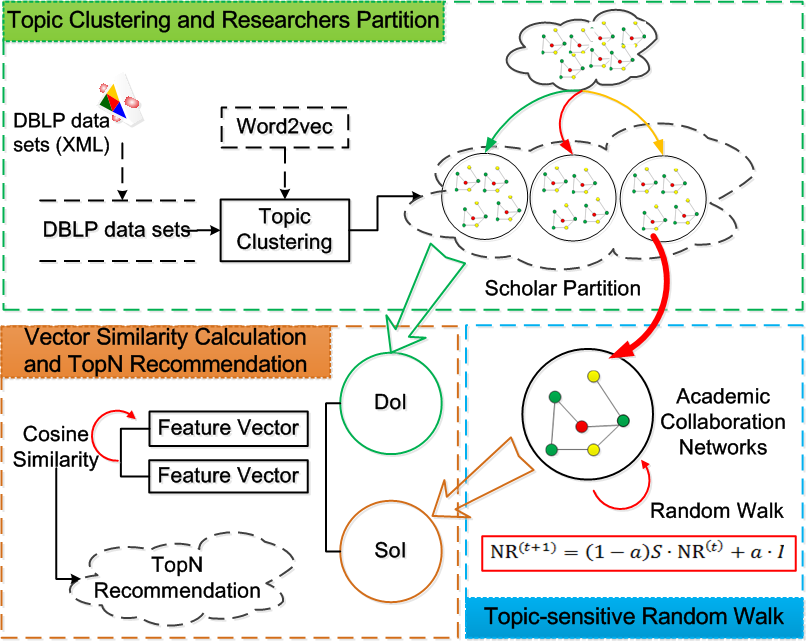
\includegraphics [width=3.4in]{Fig1.png}
\caption{The architecture diagram of CCRec model}
\end{figure}

Figure 1 depicts the four components of CCRec: \textit{topic clustering and researcher partition}, \textit{Topic-sensitive random walk}, \textit{vector similarity calculation and TopN recommendation}. Topic clustering and researcher partition distribute researchers according to multiple domains and get a DoI for each researcher. Topic-sensitive random walk calculates the SoI in each domain. And the TopN recommendation gives the recommending list.

\subsection{Topic Clustering and researcher Partition}
% -----------------------------------------------------------------------------
In CCRec, topic clustering and researcher partition generate various domains and map all researchers into these domains. Initially, CCRec extract keywords from titles of all the papers for each researcher, meanwhile filtering out some meaningless words, e.g. "of","the", "and", etc. As a core text for a paper, these keywords preprocessed are rich in a variety of academic topics. We use word2vec, a famous tool of NLP (Natural Language Processing) to cluster the keywords into various domains. Then, if some keywords of a researcher belong to a domain, we will partition the researcher to this domain. What we should emphasis is that one researcher always belongs to several domains and there are also a great many researchers in one domain.

\subsection{Feature Vector Calculation}
% -----------------------------------------------------------------------------
To measure the distribution of researchers' interest, we define DoI as researcher's proportion of interest in one domain:
\begin{equation}
DoI_{s,d}=\frac{N_{d}}{\sum_{k=1}^{n} N_{k}}
\end{equation}
Where $N_{d}$ is the number of key words of researcher $s$ in domain $d$. It is a content-based method by utilizing the information on the titles of researchers' publications.

We define SoI as researcher's strength of influence in one domain, which is measured by a topic-sensitive random walk method based on collaboration networks. The core equation of the random walk method is shown follow:
\begin{equation}
R_{d}^{(t+1)}=\alpha \mathbf{S}R_{d}^{(t)}+(1-\alpha)q
\end{equation}
Where $R_{d}$ represent the rank score vector of all researchers in domain $d$, $q$ is the initial vector of $R$, $\alpha$ denotes the damping coefficient. Random walk is a iterative process. After limited iterations, the vector $R$ will be convergent. The vector item is $SoI$ here. We can get $SoI_{s}=R_{d,s}$.

To be more accurate, We define feature vector $F$ by combining $DoI$ and $SoI$, which measures the academic feature of researchers on various domains.

\begin{equation}
F_{s,d}=DoI_{s}*SoI_{s}
\end{equation}

\subsection{Collaboration Recommendation by Feature Vector Similarity}
% -----------------------------------------------------------------------------
In CCRec, The academic feature of researchers is measured by the feature vector $F$. We use a \emph{cosine similarity} method to compute the similarity of these feature vectors, and further denoting the similarity between researchers.
\begin{equation}
Sim(s_{1},s_{2})=\frac{\sum_{i=1}^{n}(F_{s_{1},i}*F_{s_{2},i})}{\sqrt{\sum_{i=1}^{n}F_{s_{1},i}^2}*\sqrt{\sum_{i=1}^{n}F_{s_{2},i}^2}}
\end{equation}

Finally, CCRec recommends to researchers those potential collaborators who have high similarity with them, and provide a TopN collaborators recommendation list.
% =============================================================================
\section{Evaluation and Analysis}
% =============================================================================
\begin{figure*}
\centering
\subfigure[Precision]{
\label{fig:2-a}
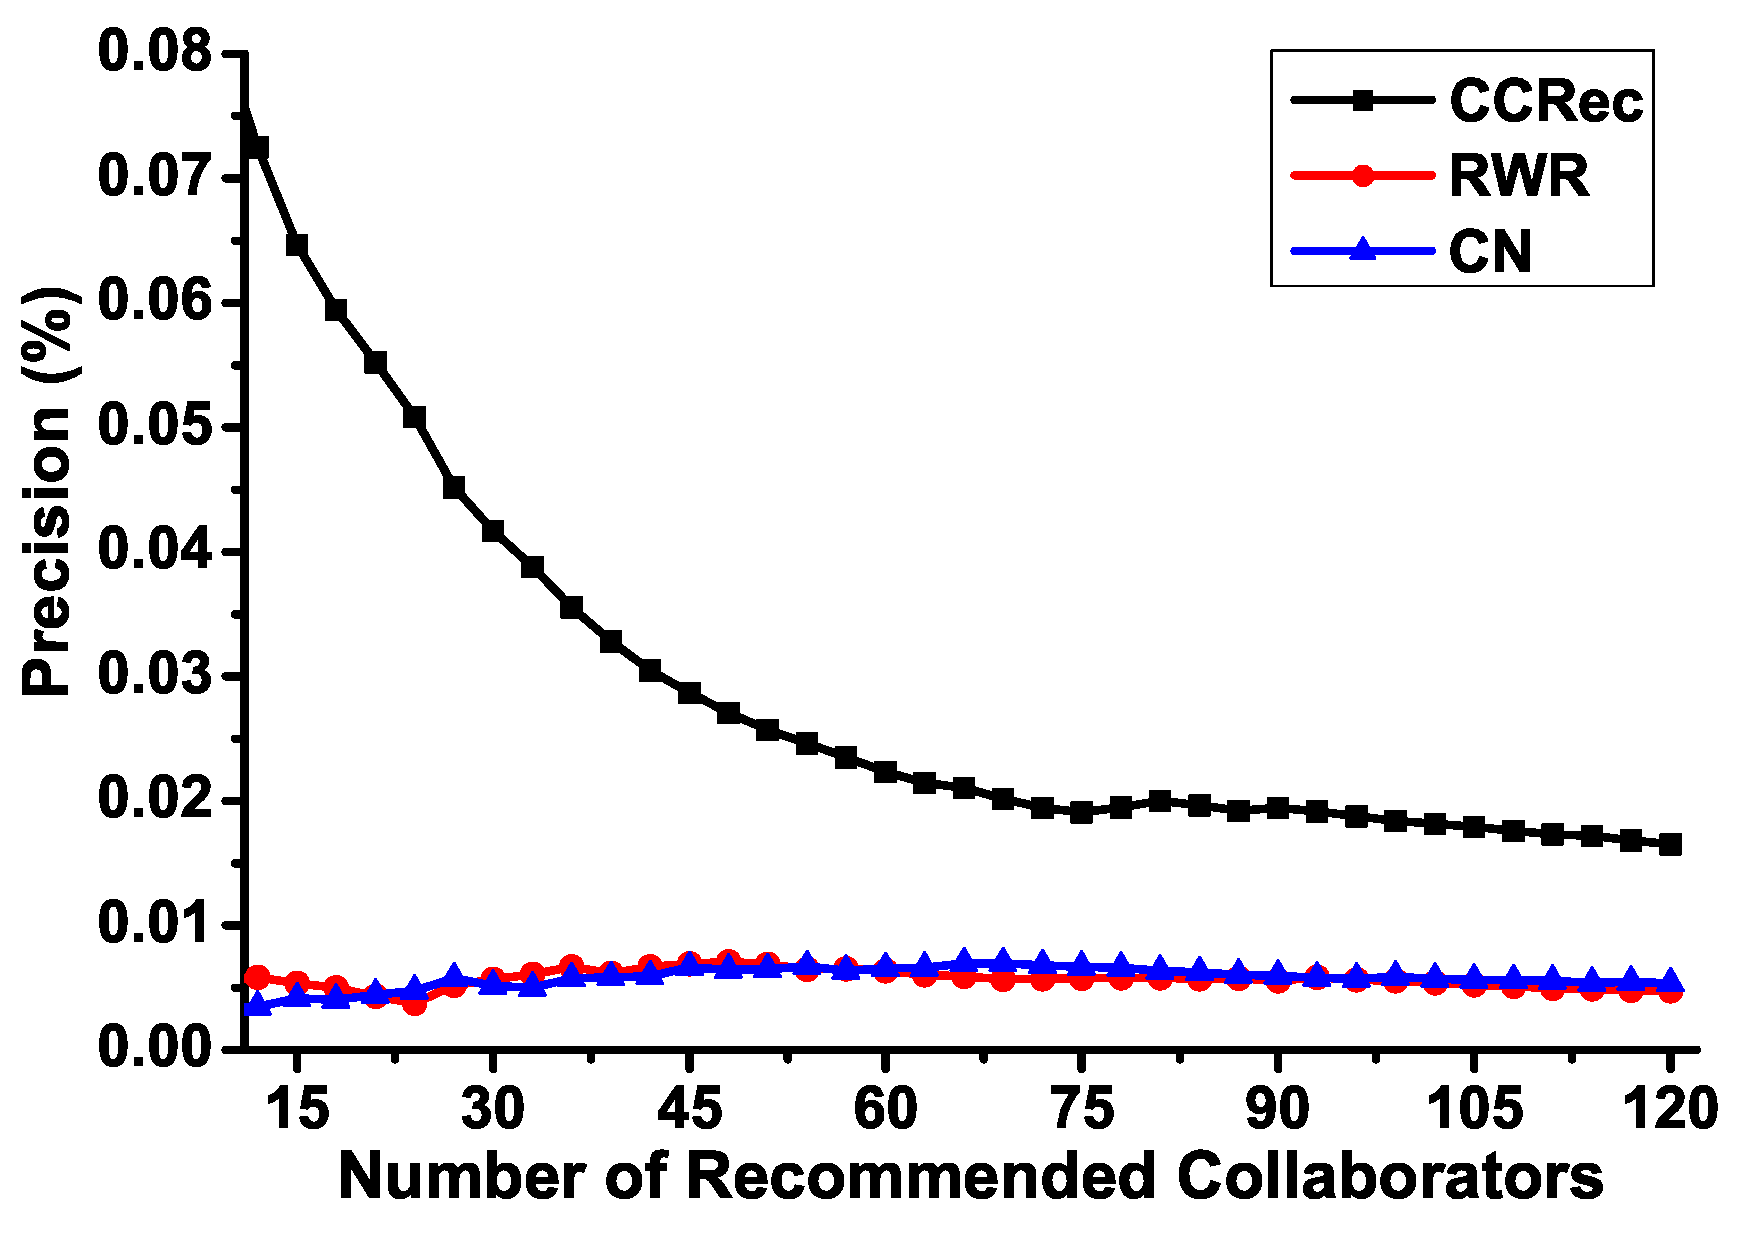
\includegraphics[width=0.32\textwidth]{Fig2-a.eps}}
\subfigure[Recall Rate]{
\label{fig:2-b}
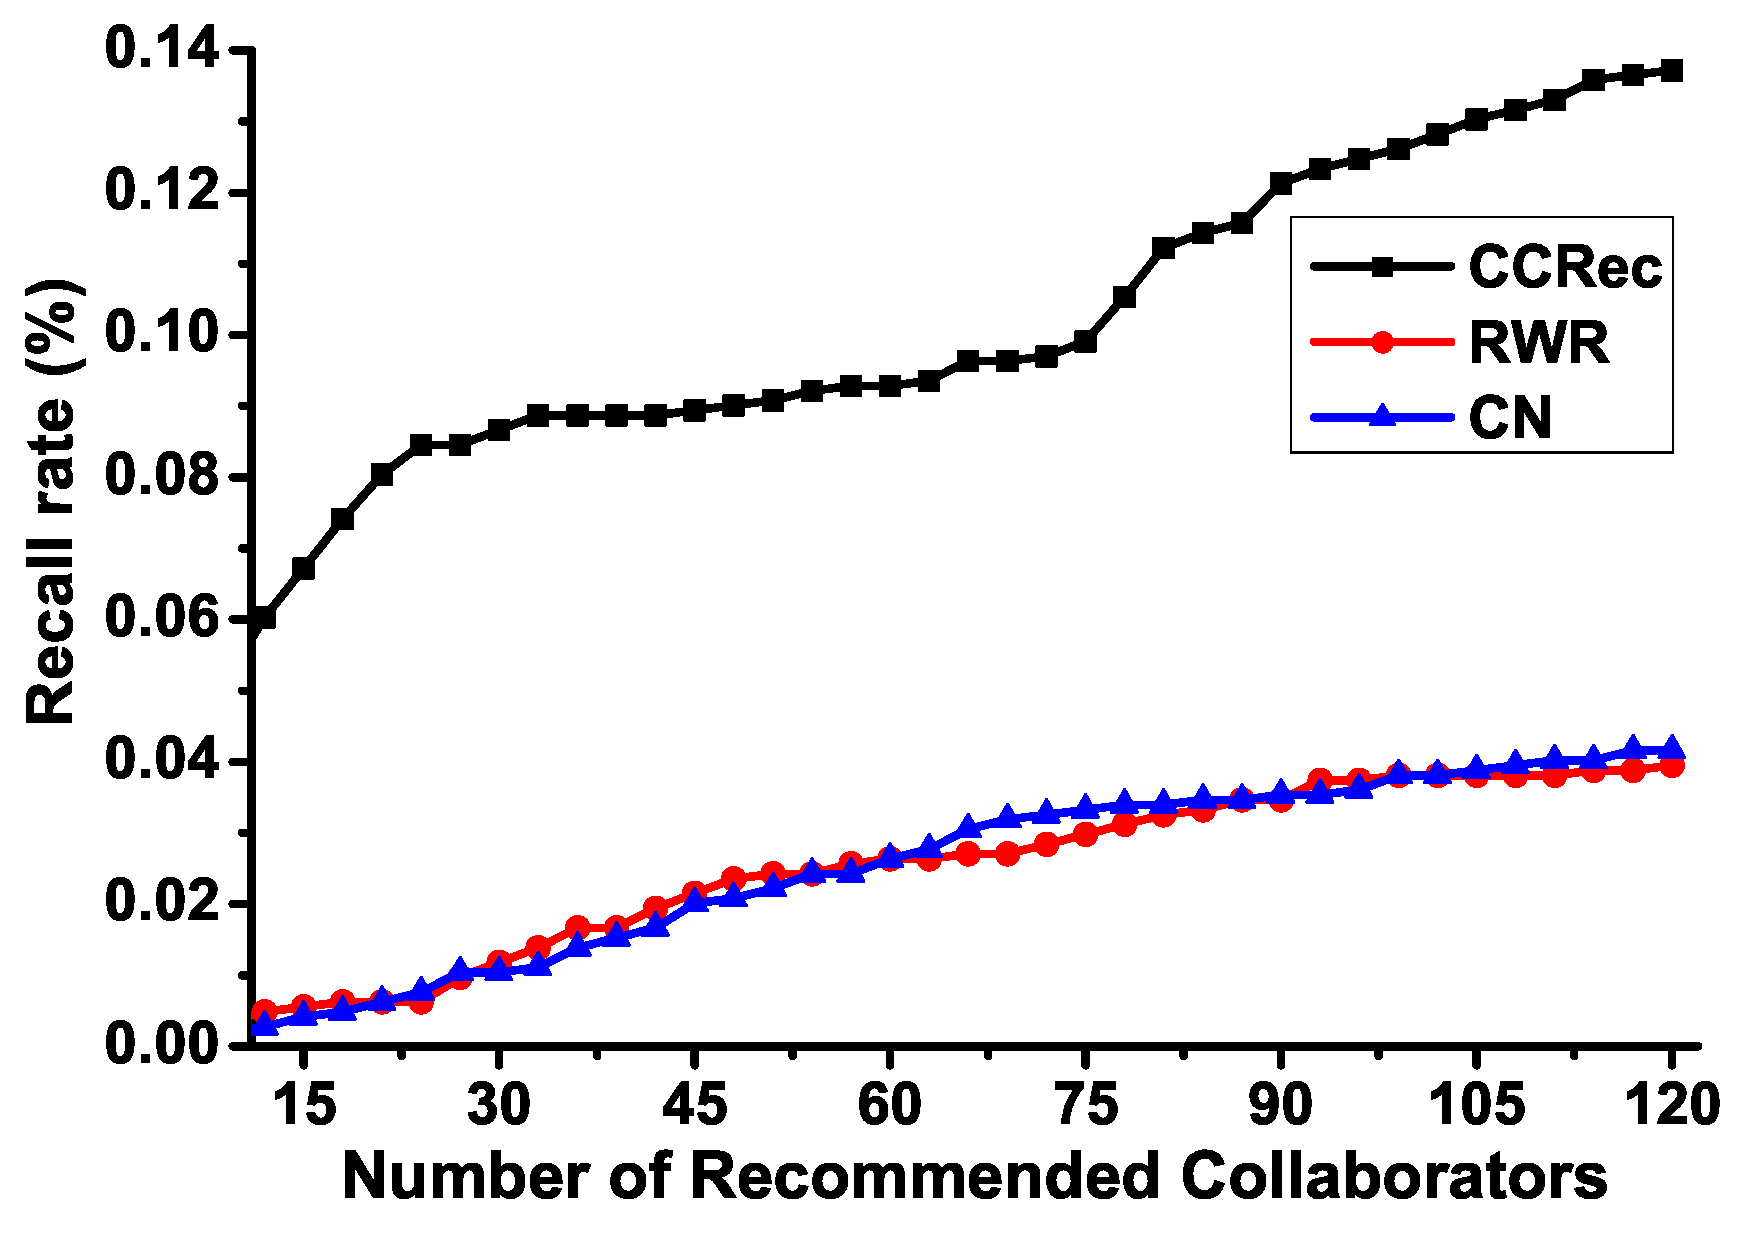
\includegraphics[width=0.32\textwidth]{Fig2-b.eps}}
\subfigure[F1]{
\label{fig:2-c}
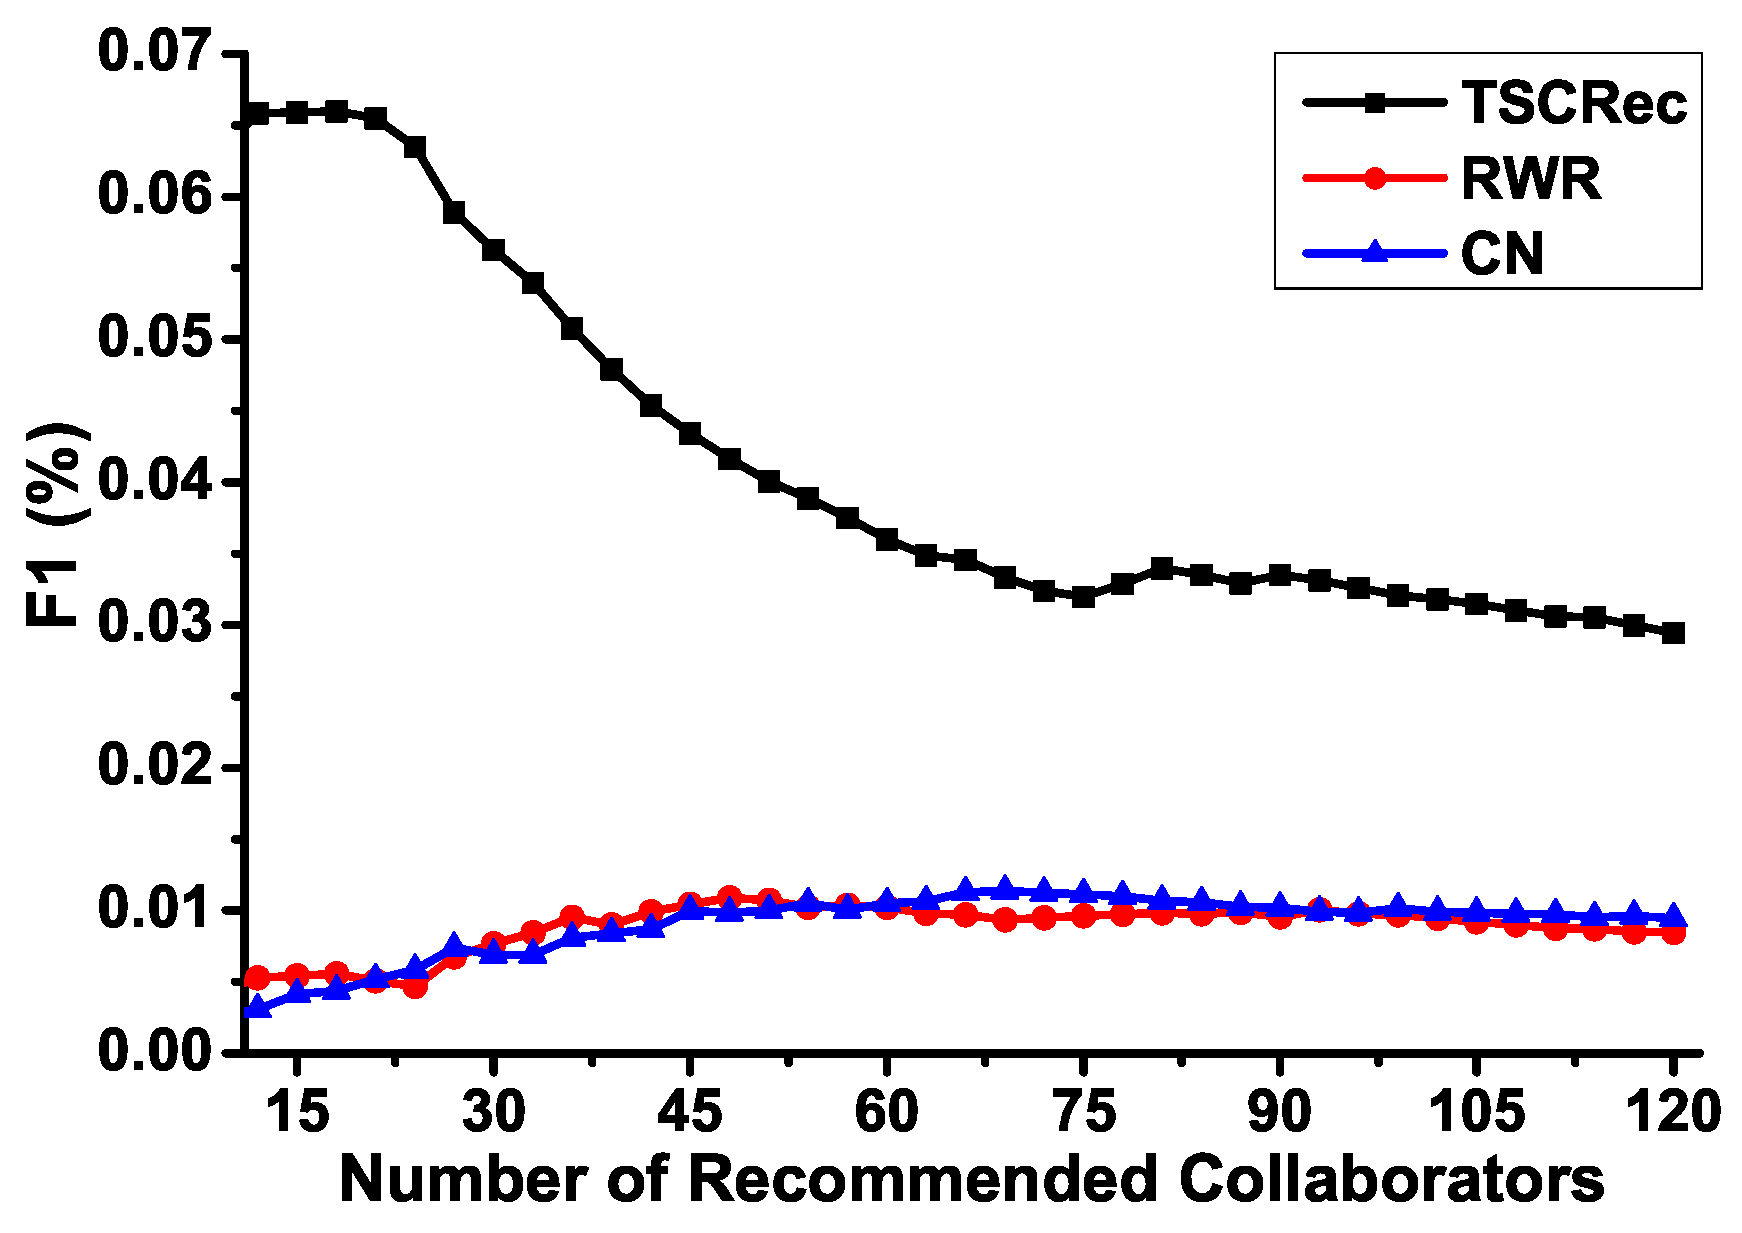
\includegraphics[width=0.32\textwidth]{Fig2-c.eps}}
\caption{Performance of CCRec, RWR and FOF}
\label{fig:5}       % Give a unique label
\end{figure*}
We have conducted experiments based on a subset of DBLP data, which relevant to data mining. We take the year 2011 as the partition time of training set and testing set. To better evaluate our model, we compared CCRec with two traditional approaches Random Walk with Restart (RWR) and Common Neighbors (CN) \cite{li2014acrec}. We adopt three metrics to evaluate the performance, precision, recall rate and F1. What we should illustrate is that we recommend the new collaborators who never cooperated with the target researcher, because the new collaborators are more meaningful and practical in real academic filed.

Figure 2 shows the performance of CCRec, RWR and CN in precision, recall rate and F1 with the number of recommended collaborators increasing. It can be observed that CCRec significantly outperforms RWR and CN. For these three metrics, CCRec exceeds RWR and CN all the time. CCRec shows a downtrend for precision and an uptrend for recall rate. For the F1, it reaches the peak 6.598\% when recommending 18 researchers, which can be regarded as an best point.

Figure 2-a reveals that the precision of CCRec is always higher than that of RWR and CN. It shows an upward tendency for the recall rate of CCRec, which is obviously superior to RWR and CN. For the F1, CCRec exceeds RWR and CN all the time, and

In short, CCRec outperforms RWR and CN with higher precision, recall rate and F1. This is because CCRec with content of publications and collaboration network combined has a distinct advantage in recommending new collaborators.

% =============================================================================
\section{Conclusion}
% =============================================================================
The conclusions we reach are: 1) CCRec outperforms RWR and CN in precision, recall rate and F1 integrating the content of publications with academic collaboration network. 2) With topic clustering, the problem of topic drift has been well solved.

Our research on CCRec reveals that, combining the information of publications' content and collaboration networks can do help to recommend collaborators better and make collaboration recommendation be more specific and effective.

\balance
\bibliographystyle{acm-sigchi}
\bibliography{CCRec}

\end{document}
